\documentclass[11pt]{article}
\usepackage{amsmath, amssymb, physics, mathtools, bm}
\usepackage{tikz, pgfplots}
\pgfplotsset{compat=1.18}
\usepackage[margin=2.3cm]{geometry}
\usepackage{siunitx, booktabs, hyperref}
\newcommand{\D}{\mathrm{D}}
\newcommand{\de}{\mathrm{d}}
\newcommand{\pd}[2]{\frac{\partial #1}{\partial #2}}
\newcommand{\pdd}[2]{\frac{\partial^{2} #1}{\partial #2^{2}}}
\newcommand{\Lap}{\nabla^{2}}
\title{B1 Fluids, 2025 --- Model Solutions}
\author{}
\date{}
\begin{document}
\maketitle

%==============================================================
\section*{Question 1 --- Streamfunction, vorticity and point vortices}

\textbf{Problem statement.} Introduce the streamfunction $\psi$ for 2D incompressible flow and prove the Bernoulli--vorticity relations $\omega=\omega(\psi)$, $B=B(\psi)$, $\omega=-\de B/\de\psi$. Apply to a Rankine vortex, and to two point vortices of strengths $A$ and $B$.

\subsection*{(a) Continuity, streamfunction and vorticity}

Continuity for a compressible fluid:
\begin{equation}
\pd{\rho}{t} + \nabla\cdot(\rho\vb v) = 0.
\end{equation}
Incompressibility ($\D\rho/\D t=0$) reduces this to
\[ \nabla\cdot\vb v = 0. \]
In 2D, $\partial_x v_x + \partial_y v_y = 0$ is the integrability condition for $\psi(x,y)$ with
\[ v_x = -\pd{\psi}{y},\qquad v_y = \pd{\psi}{x}, \]
i.e.\ $\vb v = -\hat{\vb z}\times\nabla\psi$. The vorticity $\bm\omega = \omega\hat{\vb z}$ has
\begin{equation}
\boxed{\;\omega = \pdd{\psi}{x} + \pdd{\psi}{y} = \nabla^{2}\psi.\;}
\end{equation}
Lines of constant $\psi$ are streamlines since $\vb v\cdot\nabla\psi = 0$.

\subsection*{(b) Bernoulli--vorticity theorem for steady 2D inviscid flow}

Euler:
\begin{equation}
\pd{\vb v}{t} + (\vb v\cdot\nabla)\vb v = -\frac{1}{\rho}\nabla p - g\hat{\vb z}.
\label{eq:euler}
\end{equation}
Using $(\vb v\cdot\nabla)\vb v = \nabla(\tfrac12 v^2) - \vb v\times(\nabla\times\vb v)$, steady flow in a horizontal plane (gravity absorbed into $p$):
\[ \nabla\!\left(\frac{p}{\rho}+\frac{v^2}{2}\right) = \vb v\times(\omega\hat{\vb z}) = \omega\nabla\psi, \]
since $\vb v\times\hat{\vb z} = \nabla\psi$. With $B\equiv p/\rho + \tfrac12 v^2$,
\begin{equation}
\nabla B = \omega\nabla\psi.
\label{eq:nablaB}
\end{equation}
Dotting with $\vb v\perp\nabla\psi$ gives $\vb v\cdot\nabla B=0$, so
\begin{equation}
\boxed{\;B = B(\psi).\;}
\end{equation}
Curl of \eqref{eq:euler} kills both gradient terms, so $\D\omega/\D t=0$; in steady flow,
\begin{equation}
\boxed{\;\omega = \omega(\psi).\;}
\end{equation}
Substituting $\nabla B = (\de B/\de\psi)\nabla\psi$ in \eqref{eq:nablaB} and fixing the sign by the rigid-rotation check ($\psi=-\tfrac12\Omega r^2$, $\omega=2\Omega$):
\begin{equation}
\boxed{\;\omega = -\frac{\de B}{\de\psi}.\;}
\end{equation}

\subsection*{(c) Rankine vortex}

Symmetry gives $\vb v = v_\theta(r)\hat{\bm\theta}$ and
\[ \omega = \frac{1}{r}\dv{r}(rv_\theta). \]
Inside ($r\le r_0$, $\omega=\omega_0$), regularity at $r=0$:
\[ v_\theta = \tfrac12\omega_0 r. \]
Outside ($\omega=0$), $rv_\theta=$ const; matching at $r_0$:
\begin{equation}
\boxed{\;v_\theta(r) = \begin{cases}\tfrac12\omega_0 r, & r\le r_0,\\[2pt] \tfrac12\omega_0 r_0^2/r, & r>r_0.\end{cases}\;}
\label{eq:v-rankine}
\end{equation}
Radial Euler (centripetal balance):
\[ \frac{1}{\rho}\dv{p}{r} = \frac{v_\theta^2}{r}. \]
Outside, substitute $v_\theta = \omega_0 r_0^2/(2r)$:
\[ \frac{v_\theta^2}{r} = \frac{\omega_0^2 r_0^4}{4 r^3}. \]
Integrate from $r$ to $\infty$ with $p(\infty)=p_\infty$:
\[ p_\infty - p(r) = \int_r^\infty \frac{\rho\omega_0^2 r_0^4}{4 r'^3}\,\de r' = \frac{\rho\omega_0^2 r_0^4}{8 r^2}. \]
Hence outside,
\[ p(r) = p_\infty - \frac{\rho\omega_0^2 r_0^4}{8 r^2}. \]
Inside, substitute $v_\theta = \tfrac12\omega_0 r$:
\[ \frac{v_\theta^2}{r} = \tfrac14\omega_0^2 r. \]
Integrate:
\[ p(r) = \tfrac18\rho\omega_0^2 r^2 + C. \]
Apply continuity at $r=r_0$:
\[ \tfrac18\rho\omega_0^2 r_0^2 + C = p_\infty - \tfrac18\rho\omega_0^2 r_0^2. \]
Solve for $C$:
\[ C = p_\infty - \tfrac14\rho\omega_0^2 r_0^2. \]
Therefore
\begin{equation}
\boxed{\;p(r) = \begin{cases}\,p_\infty - \tfrac14\rho\omega_0^2 r_0^2 + \tfrac18\rho\omega_0^2 r^2, & r\le r_0,\\[3pt] p_\infty - \dfrac{\rho\omega_0^2 r_0^4}{8 r^2}, & r>r_0.\end{cases}\;}
\end{equation}

\subsection*{(d) Two point vortices}

Each vortex moves only in the field of the other. With separation $\vb d=\vb x_2-\vb x_1$, $L=|\vb d|$:
\begin{equation}
\dot{\vb x}_1 = \frac{B}{2\pi L^2}\hat{\vb z}\times\vb d,\qquad \dot{\vb x}_2 = -\frac{A}{2\pi L^2}\hat{\vb z}\times\vb d.
\end{equation}
Hence
\begin{equation}
\dot{\vb d} = -\frac{A+B}{2\pi L^2}\hat{\vb z}\times\vb d,\qquad A\vb x_1 + B\vb x_2 = \text{const}.
\label{eq:com-conserved}
\end{equation}
Since $\dot{\vb d}\perp\vb d$, $L$ is constant.

\paragraph{Case $A=B$.} Centroid fixed; both vortices co-rotate about the midpoint on circles of radius $L/2$.

\paragraph{Case $A=-B$.} $\dot{\vb d}=0$; \eqref{eq:com-conserved} gives equal translational velocity $\dot{\vb x}_1=\dot{\vb x}_2 = (B/2\pi L^2)\hat{\vb z}\times\vb d$. Pair propagates as two parallel straight lines.

\paragraph{Sketch.}
\begin{center}
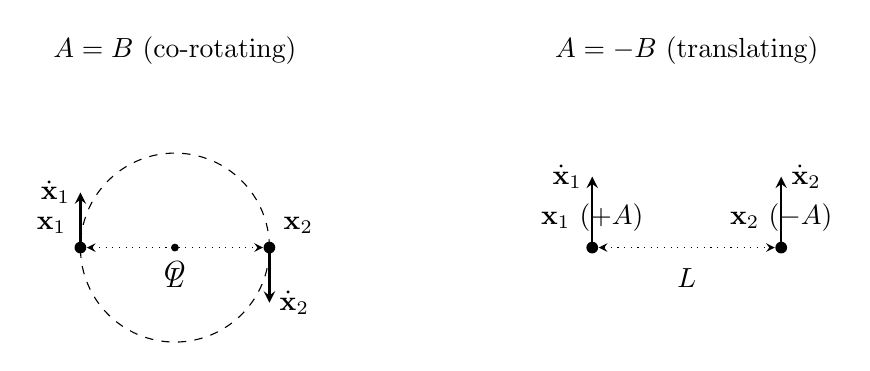
\begin{tikzpicture}[>=stealth, scale=1.0]
  % Case A=B: co-rotating pair
  \draw[dashed] (0,0) circle (1.2);
  \node[circle,fill,inner sep=1.5pt,label=above left:{$\vb x_1$}] (V1) at (-1.2,0) {};
  \node[circle,fill,inner sep=1.5pt,label=above right:{$\vb x_2$}] (V2) at ( 1.2,0) {};
  \node[circle,fill,inner sep=1.0pt,label=below:{$O$}] at (0,0) {};
  \draw[<->,dotted] (V1) -- (V2) node[midway,below=4pt] {$L$};
  \draw[->,thick] (-1.2,0) -- (-1.2,0.7) node[left] {$\dot{\vb x}_1$};
  \draw[->,thick] ( 1.2,0) -- ( 1.2,-0.7) node[right] {$\dot{\vb x}_2$};
  \node[above=1.0cm] at (0,1.2) {$A=B$ (co-rotating)};

  % Case A = -B: translating pair
  \begin{scope}[xshift=6.5cm]
    \node[circle,fill,inner sep=1.5pt,label=above:{$\vb x_1$ ($+A$)}] (W1) at (-1.2,0) {};
    \node[circle,fill,inner sep=1.5pt,label=above:{$\vb x_2$ ($-A$)}] (W2) at ( 1.2,0) {};
    \draw[<->,dotted] (W1) -- (W2) node[midway,below=4pt] {$L$};
    \draw[->,thick] (-1.2,0) -- (-1.2,0.9) node[left] {$\dot{\vb x}_1$};
    \draw[->,thick] ( 1.2,0) -- ( 1.2,0.9) node[right] {$\dot{\vb x}_2$};
    \node[above=1.0cm] at (0,1.2) {$A=-B$ (translating)};
  \end{scope}
\end{tikzpicture}
\end{center}

\paragraph{Frequency (periodic case $A=B$).} From \eqref{eq:com-conserved}, $|\dot{\vb d}|=\Omega L$ with $\Omega = (A+B)/(2\pi L^2)$:
\begin{equation}
\boxed{\;\omega_{\text{orb}} = \frac{A+B}{2\pi L^2} = \frac{A}{\pi L^2}\quad(A=B).\;}
\end{equation}

%==============================================================
\section*{Question 2 --- Complex potential and conformal mappings}

\textbf{Problem statement.} For analytic $w(z)=\phi+\mathrm{i}\psi$, derive Cauchy--Riemann, harmonicity and orthogonality of level curves. Apply to $w=Bz^2$. Define a conformal mapping; invert $Z = z/2 + \sqrt{z^2/4-c^2}$ and find $\Phi,\Psi$ for $w(z)=Az$ in the $Z$-plane.

\subsection*{(a) Analytic functions and Cauchy--Riemann}

Analytic $w$: $w'(z)$ direction-independent. Equating $\Delta z=\Delta x$ and $\Delta z=\mathrm{i}\Delta y$ limits,
\[ w'(z) = \pd{\phi}{x}+\mathrm{i}\pd{\psi}{x} = -\mathrm{i}\pd{\phi}{y}+\pd{\psi}{y}. \]
Real/imaginary parts:
\begin{equation}
\boxed{\;\pd{\phi}{x}=\pd{\psi}{y},\qquad \pd{\phi}{y}=-\pd{\psi}{x}.\;}
\label{eq:CR}
\end{equation}
Cross-differentiating \eqref{eq:CR},
\[ \Lap\phi = 0,\qquad \Lap\psi = 0. \]
Orthogonality:
\[ \nabla\phi\cdot\nabla\psi = (\partial_y\psi)(\partial_x\psi) + (-\partial_x\psi)(\partial_y\psi) = 0. \]
For 2D incompressible irrotational inviscid flow, $\phi$ is the velocity potential ($\vb v=\nabla\phi$) and $\psi$ the streamfunction; \eqref{eq:CR} reproduces $v_x=\partial_x\phi=\partial_y\psi$, $v_y=\partial_y\phi=-\partial_x\psi$.

\subsection*{(b) The flow $w(z)=Bz^2$}

$w = B(x^2-y^2) + 2\mathrm{i}Bxy$, so
\begin{equation}
\boxed{\;\phi = B(x^2-y^2),\qquad \psi = 2Bxy.\;}
\end{equation}
Streamlines $\psi=$ const are hyperbolae $xy=$ const ($\psi=0$ is the axes); equipotentials $x^2-y^2=$ const are the orthogonal family.
\begin{center}
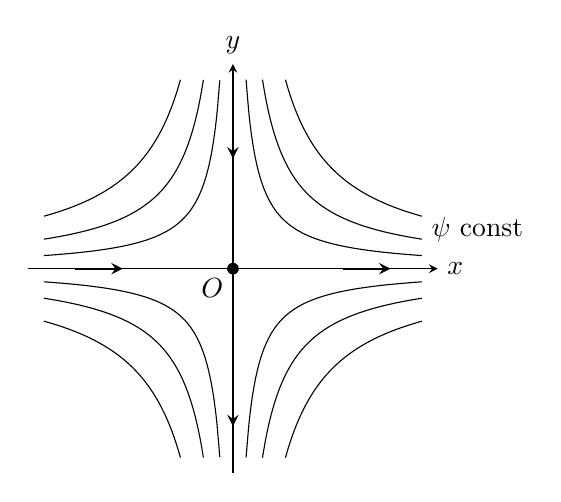
\begin{tikzpicture}[>=stealth, scale=1.0]
  \draw[->] (-2.6,0) -- (2.6,0) node[right] {$x$};
  \draw[->] (0,-2.6) -- (0,2.6) node[above] {$y$};
  % Streamlines xy = const in each quadrant
  \foreach \k in {0.4,0.9,1.6} {
    \draw[domain=\k/2.4:2.4, smooth, samples=60] plot (\x, \k/\x);
    \draw[domain=-2.4:-\k/2.4, smooth, samples=60] plot (\x, \k/\x);
    \draw[domain=\k/2.4:2.4, smooth, samples=60] plot (\x, -\k/\x);
    \draw[domain=-2.4:-\k/2.4, smooth, samples=60] plot (\x, -\k/\x);
  }
  % Stagnation point
  \node[circle,fill,inner sep=1.5pt] at (0,0) {};
  \node[below left] at (0,0) {$O$};
  % Flow direction arrows (B>0): along +y axis downward, +x axis outward
  \draw[->,thick] (0,2.0) -- (0,1.4);
  \draw[->,thick] (1.4,0) -- (2.0,0);
  \draw[->,thick] (0,-1.4) -- (0,-2.0);
  \draw[->,thick] (-2.0,0) -- (-1.4,0);
  \node[right] at (2.4,0.5) {$\psi$ const};
\end{tikzpicture}
\end{center}
For $B>0$: in the first quadrant fluid descends along the $+y$ axis and exits along the $+x$ axis.

Velocity: $u-\mathrm{i}v = w'(z) = 2Bz$, so $\vb v = (2Bx,-2By)$. The point $w'(z)=0$ at $z=0$ is a stagnation point: 2D corner-flow saddle, fluid against a right-angled wall.

\subsection*{(c) Conformal mapping and Joukowski plate}

A holomorphic $Z=f(z)$ with $f'\ne 0$ is a conformal map: angles preserved. If $w(z)$ is analytic then $W(Z)\equiv w(F(Z))$ with $z=F(Z)$ is analytic in $Z$ and represents another potential flow; streamlines map by $f$.

Invert $Z = z/2 + \sqrt{z^2/4-c^2}$. Subtract $z/2$:
\[ Z - \tfrac{z}{2} = \sqrt{\tfrac{z^2}{4}-c^2}. \]
Square both sides:
\[ \left(Z-\tfrac{z}{2}\right)^2 = \tfrac{z^2}{4}-c^2. \]
Expand the left-hand side:
\[ Z^2 - zZ + \tfrac{z^2}{4} = \tfrac{z^2}{4}-c^2. \]
Cancel $z^2/4$:
\[ Z^2 - zZ = -c^2. \]
Solve for $z$:
\[ zZ = Z^2 + c^2. \]
Divide by $Z$:
\begin{equation}
\boxed{\;z = F(Z) = Z + \frac{c^2}{Z}.\;}
\end{equation}
On $|Z|=c$, write $Z=c\mathrm{e}^{\mathrm{i}\theta}$:
\[ z = c\mathrm{e}^{\mathrm{i}\theta} + c\mathrm{e}^{-\mathrm{i}\theta} = 2c\cos\theta \in [-2c,2c]. \]

For $w(z)=Az$ (uniform stream of speed $A$),
\[ W(Z) = A\!\left(Z + \frac{c^2}{Z}\right). \]
With $Z=R\mathrm{e}^{\mathrm{i}\Theta}$,
\begin{equation}
\boxed{\;\Phi = A\!\left(R+\frac{c^2}{R}\right)\cos\Theta,\qquad \Psi = A\!\left(R-\frac{c^2}{R}\right)\sin\Theta.\;}
\label{eq:Phi-Psi}
\end{equation}
$\Psi=0$ on the real axis or on $R=c$: \eqref{eq:Phi-Psi} is uniform flow past a rigid cylinder of radius $c$. In the $z$-plane the cylinder collapses to the flat plate $z\in[-2c,2c]$, so $w=Az$ in $z$ is uniform flow past a horizontal flat plate of length $4c$.

\paragraph{Real fluid.} Viscosity enforces no-slip, generating a boundary layer that separates on the rear half at large Re, producing a wake and finite drag (resolving d'Alembert's paradox). The wake is unsteady (von K\'arm\'an street), so the symmetric streamlines of \eqref{eq:Phi-Psi} are never observed near the body; the conformal result describes only the outer irrotational flow.

%==============================================================
\section*{Question 3 --- Thin viscous film on an inclined conveyor belt}

\textbf{Problem statement.} A thin viscous film $h(x,t)$ on a belt inclined at $\theta$, moving at $U_0\hat{\vb x}$; $y$ normal to belt. Define Re, derive the lubrication equation, find $v_x(y)$, the equilibrium thickness, and timescales after the belt stops.

\subsection*{(a) Reynolds number and lubrication}

\[ \mathrm{Re} = \frac{|(\vb v\cdot\nabla)\vb v|}{|\nu\nabla^2\vb v|} \sim \frac{UL}{\nu}. \]
Re$\,\ll 1$: viscous diffusion dominates (Stokes). For a thin film, aspect ratio $\epsilon = h/L\ll 1$; incompressibility gives $v_y\sim\epsilon U_0$, and the inertial term is smaller than $\nu\partial_y^2 v_x$ by $\epsilon\,\mathrm{Re}\ll 1$:
\begin{equation}
0 = -\frac{1}{\rho}\pd{p}{x} + g\sin\theta + \nu\pdd{v_x}{y},\qquad 0 = -\frac{1}{\rho}\pd{p}{y} - g\cos\theta.
\label{eq:NS-lub}
\end{equation}
Streamwise viscous term $\nu\partial_x^2 v_x$ suppressed by $\epsilon^2$.

Integrate \eqref{eq:NS-lub}$_2$ in $y$:
\[ p(x,y) = -\rho g\cos\theta\,y + f(x). \]
Apply $p(y=h)=p_a$ (no surface tension):
\[ f(x) = p_a + \rho g\cos\theta\,h(x). \]
Hence
\[ p = p_a + \rho g\cos\theta\,(h-y). \]
Differentiate with respect to $x$:
\[ \pd{p}{x} = \rho g\cos\theta\,\pd{h}{x}. \]
Substitute into \eqref{eq:NS-lub}$_1$:
\begin{equation}
\boxed{\;g\pd{h}{x}\cos\theta + g\sin\theta = \nu\pdd{v_x}{y}.\;}
\label{eq:lubrication}
\end{equation}

\subsection*{(b) Boundary conditions and velocity profile}

No-slip at belt; no tangential stress at the free surface:
\[ v_x(0) = U_0,\qquad \eval{\pd{v_x}{y}}_{y=h} = 0. \]
Write $G \equiv g\cos\theta\,\partial h/\partial x + g\sin\theta$, so \eqref{eq:lubrication} reads $\nu\,\partial^2 v_x/\partial y^2 = G$. Integrate once in $y$:
\[ \nu\pd{v_x}{y} = Gy + C_1. \]
Apply $\partial_y v_x|_{y=h}=0$:
\[ C_1 = -Gh. \]
So
\[ \nu\pd{v_x}{y} = G(y-h). \]
Integrate again:
\[ \nu v_x = G\!\left(\tfrac12 y^2 - hy\right) + C_2. \]
Apply $v_x(0)=U_0$:
\[ C_2 = \nu U_0. \]
Therefore
\begin{equation}
\boxed{\;v_x(x,y,t) = U_0 + \frac{1}{\nu}\!\left[g\cos\theta\,\pd{h}{x} + g\sin\theta\right]\!\left(\tfrac12 y^2 - hy\right).\;}
\label{eq:vx-profile}
\end{equation}

\subsection*{(c) Equilibrium thickness}

Steady, $\partial h/\partial x = 0$:
\begin{equation}
v_x(y) = U_0 + \frac{g\sin\theta}{\nu}\!\left(\tfrac12 y^2 - h_{\text{eq}} y\right).
\label{eq:vx-eq}
\end{equation}
Flux per unit width:
\[ Q = \int_0^{h_{\text{eq}}}\!\!v_x\,\de y. \]
Substitute \eqref{eq:vx-eq}:
\[ Q = \int_0^{h_{\text{eq}}}\!\!\left[U_0 + \frac{g\sin\theta}{\nu}\!\left(\tfrac12 y^2 - h_{\text{eq}} y\right)\right]\de y. \]
Integrate term by term:
\[ Q = U_0 h_{\text{eq}} + \frac{g\sin\theta}{\nu}\!\left(\tfrac16 h_{\text{eq}}^3 - \tfrac12 h_{\text{eq}}^3\right). \]
Simplify:
\[ Q = U_0 h_{\text{eq}} - \frac{g\sin\theta\,h_{\text{eq}}^3}{3\nu}. \]
Impose no net transport, $Q=0$:
\[ U_0 = \frac{g\sin\theta\,h_{\text{eq}}^2}{3\nu}. \]
Solve for $h_{\text{eq}}$:
\begin{equation}
\boxed{\;h_{\text{eq}} = \sqrt{\frac{3\nu U_0}{g\sin\theta}}.\;}
\label{eq:heq}
\end{equation}
At $y=h_{\text{eq}}$, using $g\sin\theta\,h_{\text{eq}}^2/\nu = 3U_0$:
\[ v_x(h_{\text{eq}}) = U_0 + 3U_0\!\left(\tfrac12 - 1\right) = U_0 - \tfrac32 U_0 = -\tfrac12 U_0. \]
Zero-crossing $v_x=0$ at $y_* = h_{\text{eq}}(1-1/\sqrt 3)\approx 0.42\,h_{\text{eq}}$.
\begin{center}
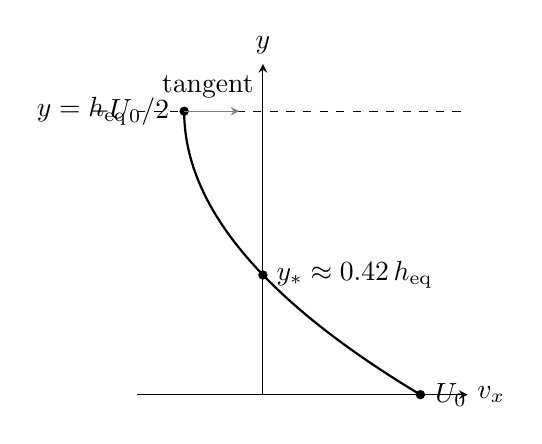
\begin{tikzpicture}[>=stealth, scale=1.0]
  \draw[->] (0,0) -- (0,4.2) node[above] {$y$};
  \draw[->] (-1.6,0) -- (2.6,0) node[right] {$v_x$};
  \draw[dashed] (-1.6,3.6) -- (2.6,3.6);
  \node[left] at (-1.6,3.6) {$y=h_{\text{eq}}$};
  % Parabola: v_x(y) = U_0 + (g sin theta / nu)(y^2/2 - h_eq y); using normalised
  % Let h=3.6, U_0 -> 2.0; coefficient k so that v_x(h) = -U_0/2 = -1.0
  % v_x(y) = 2 - k*(h*y - y^2/2); at y=h: 2 - k*h^2/2 = -1 => k = 6/h^2 = 6/12.96
  \draw[thick,domain=0:3.6,smooth,samples=60,variable=\y] plot ({2 - (6/12.96)*(3.6*\y - \y*\y/2)},\y);
  \node[circle,fill,inner sep=1.2pt,label=right:{$U_0$}] at (2,0) {};
  \node[circle,fill,inner sep=1.2pt,label=left:{$-U_0/2$}] at (-1,3.6) {};
  % zero crossing y*
  \node[circle,fill,inner sep=1.2pt] at (0,1.52) {};
  \node[right] at (0.05,1.52) {$y_*\approx 0.42\,h_{\text{eq}}$};
  % horizontal tangent at top
  \draw[->,gray] (-1,3.6) -- (-0.3,3.6);
  \node[above] at (-0.7,3.65) {tangent};
\end{tikzpicture}
\end{center}

\subsection*{(d) Belt switched off}

Just after stop, no-slip gives $v_x(0)=0$; momentum redistributes via a thin viscous layer $\delta(t)\sim\sqrt{\nu t}$ at the wall while the bulk retains \eqref{eq:vx-eq}.
\begin{center}
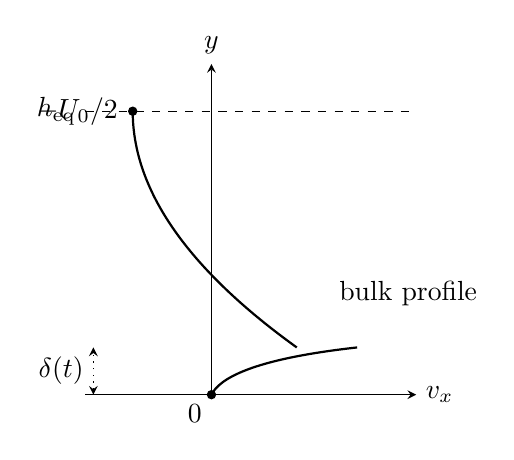
\begin{tikzpicture}[>=stealth, scale=1.0]
  \draw[->] (0,0) -- (0,4.2) node[above] {$y$};
  \draw[->] (-1.6,0) -- (2.6,0) node[right] {$v_x$};
  \draw[dashed] (-1.6,3.6) -- (2.6,3.6);
  \node[left] at (-1.6,3.6) {$h_{\text{eq}}$};
  % Bulk equilibrium parabola, but with rapid drop near y=0 to v_x=0
  \draw[thick,domain=0.6:3.6,smooth,samples=60,variable=\y] plot ({2 - (6/12.96)*(3.6*\y - \y*\y/2)},\y);
  % thin viscous layer kink: from (1.85,0.6) down to (0,0)
  \draw[thick] (1.85,0.6) .. controls (0.5,0.45) and (0.1,0.2) .. (0,0);
  \node[circle,fill,inner sep=1.2pt] at (0,0) {};
  \node[below left] at (0,0) {$0$};
  \node[circle,fill,inner sep=1.2pt,label=left:{$-U_0/2$}] at (-1,3.6) {};
  \draw[<->,dotted] (-1.5,0) -- (-1.5,0.6) node[midway,left] {$\delta(t)$};
  \node[above right] at (1.5,1.0) {bulk profile};
\end{tikzpicture}
\end{center}
\emph{Sketch (i):} equilibrium parabola with a thin viscous kink near $y=0$ pulling $v_x$ to $0$.

Once $\delta\sim h_{\text{eq}}$, the wall layer fills the film. Integrate $\nu\partial_y^2 v_x = -g\sin\theta$ once:
\[ \nu\pd{v_x}{y} = -g\sin\theta\,y + C_1. \]
Apply $\partial_y v_x(h)=0$:
\[ C_1 = g\sin\theta\,h. \]
Integrate again:
\[ \nu v_x = g\sin\theta\!\left(hy - \tfrac12 y^2\right) + C_2. \]
Apply $v_x(0)=0$:
\[ C_2 = 0. \]
Hence
\begin{equation}
v_x(y) = \frac{g\sin\theta}{\nu}\!\left(hy - \tfrac12 y^2\right).
\end{equation}
\begin{center}
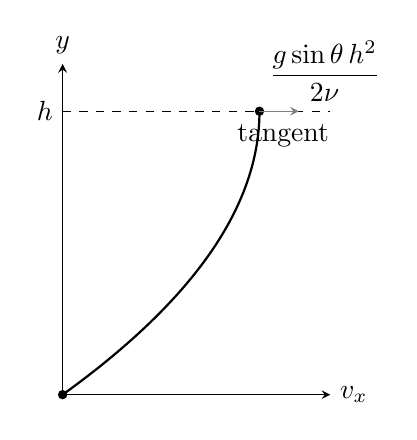
\begin{tikzpicture}[>=stealth, scale=1.0]
  \draw[->] (0,0) -- (0,4.2) node[above] {$y$};
  \draw[->] (0,0) -- (3.4,0) node[right] {$v_x$};
  \draw[dashed] (0,3.6) -- (3.4,3.6);
  \node[left] at (0,3.6) {$h$};
  % Parabola: v_x(y) ~ (hy - y^2/2); at y=h: h^2/2; pick scale so max is at x=2.5
  % v_x_norm(y) = 2.5 * (h*y - y^2/2)/(h^2/2) with h=3.6 => factor 2.5/6.48
  \draw[thick,domain=0:3.6,smooth,samples=60,variable=\y] plot ({(2.5/6.48)*(3.6*\y - \y*\y/2)},\y);
  \node[circle,fill,inner sep=1.2pt] at (0,0) {};
  \node[circle,fill,inner sep=1.2pt] at (2.5,3.6) {};
  \node[above right] at (2.5,3.6) {$\dfrac{g\sin\theta\,h^2}{2\nu}$};
  \draw[->,gray] (2.5,3.6) -- (3.0,3.6);
  \node[below] at (2.8,3.55) {tangent};
\end{tikzpicture}
\end{center}
\emph{Sketch (ii):} drainage parabola from $0$ at $y=0$ to maximum $g\sin\theta\,h^2/(2\nu)$ at $y=h$, with horizontal tangent at the free surface.

\paragraph{Diffusion timescale.} $\partial_t v_x = \nu\partial_y^2 v_x$ across $h_{\text{eq}}$:
\begin{equation}
\boxed{\;\tau_{\text{diff}} \sim \frac{h_{\text{eq}}^2}{\nu}.\;}
\end{equation}

\paragraph{Drainage timescale.} Surface speed $U_{\text{drain}}\sim g\sin\theta\,h_{\text{eq}}^2/\nu$; using \eqref{eq:heq}, $g\sin\theta\,h_{\text{eq}}^2 = 3\nu U_0$:
\begin{equation}
\boxed{\;\tau_{\text{drain}} \sim \frac{L\nu}{g\sin\theta\,h_{\text{eq}}^2} \sim \frac{L}{U_0}.\;}
\end{equation}
$\tau_{\text{drain}}/\tau_{\text{diff}} \sim L/h_{\text{eq}}\gg 1$ (lubrication limit): fast diffusion sets up the drainage profile, slow drainage empties the film.

%==============================================================
\section*{Question 4 --- Stratified instability and Rayleigh--B\'enard convection}

\textbf{Problem statement.} (a) Derive the buoyancy frequency for incompressible $\rho(z)$ and discuss instability. (b) Derive the perturbation vorticity equation and the sixth-order equation for $v_z'$ in Boussinesq Rayleigh--B\'enard. (c) For the mode $v_z'=A\sin(kx)\sin(\pi z/H)\mathrm{e}^{\sigma t}$, find $\sigma$ and the marginal Rayleigh number.

\subsection*{(a) Brunt--V\"ais\"al\"a frequency}

A parcel displaced by $\zeta$ keeps density $\rho(z_0)$; surroundings have $\rho(z_0+\zeta)\approx\rho(z_0)+\zeta\,\de\rho/\de z$. Buoyancy force per unit volume:
\[ F_b = g\zeta\,\dv{\rho}{z}. \]
Newton, $\rho(z_0)\ddot\zeta = F_b$, gives $\ddot\zeta = -\omega^2\zeta$ with
\begin{equation}
\boxed{\;\omega^2 = -\frac{g}{\rho}\dv{\rho}{z}.\;}
\end{equation}
Stable ($\de\rho/\de z<0$): oscillation. Unstable ($\de\rho/\de z>0$): $\omega^2<0$, exponential growth $\zeta\propto\mathrm{e}^{|\omega|t}$ (Rayleigh--Taylor).

\subsection*{(b) Equilibrium and perturbation equations}

Equilibrium: $\kappa\Lap T=0$, so
\begin{equation}
\boxed{\;T_{\text{eq}}(z) = T_0 - \frac{\Delta T}{H}z.\;}
\end{equation}
With $b = g\alpha(T-T_0)$, hydrostatic balance gives $p_{\text{eq}}(z) = p_0 - \rho_0 g\alpha\Delta T\,z^2/(2H)$.

Linearising $\vb v=(v_x',v_z')$, $T=T_{\text{eq}}+T'$, $p=p_{\text{eq}}+p'$:
\begin{align}
\pd{v_x'}{t} + \frac{1}{\rho_0}\pd{p'}{x} &= \nu\Lap v_x',\label{eq:pert-x}\\
\pd{v_z'}{t} - g\alpha T' + \frac{1}{\rho_0}\pd{p'}{z} &= \nu\Lap v_z',\label{eq:pert-z}\\
\pd{T'}{t} - \frac{\Delta T}{H}v_z' &= \kappa\Lap T',\label{eq:pert-T}\\
\pd{v_x'}{x} + \pd{v_z'}{z} &= 0.\label{eq:pert-cont}
\end{align}
$\partial_z$\eqref{eq:pert-x}$-\partial_x$\eqref{eq:pert-z} eliminates $p'$:
\begin{equation}
\boxed{\;\!\!\left(\pd{}{t} - \nu\Lap\right)\!\!\left(\pd{v_x'}{z} - \pd{v_z'}{x}\right) = -g\alpha\pd{T'}{x}.\;}
\label{eq:vort-final}
\end{equation}
Apply $\partial_x$ and use \eqref{eq:pert-cont} to write $\partial_x(\partial_z v_x'-\partial_x v_z') = -\Lap v_z'$:
\[ \!\!\left(\pd{}{t}-\nu\Lap\right)\Lap v_z' = g\alpha\pdd{T'}{x}. \]
Apply $(\partial_t-\kappa\Lap)$ and use \eqref{eq:pert-T} as $(\partial_t-\kappa\Lap)T' = (\Delta T/H)v_z'$:
\begin{equation}
\boxed{\;\!\!\left(\pd{}{t}-\nu\Lap\right)\!\!\left(\pd{}{t}-\kappa\Lap\right)\Lap v_z' = \frac{g\alpha\Delta T}{H}\pdd{v_z'}{x}.\;}
\label{eq:RB-master}
\end{equation}

\subsection*{(c) Normal modes and Rayleigh criterion}

For $v_z' = A\sin(kx)\sin(\pi z/H)\mathrm{e}^{\sigma t}$, $\Lap\to -K^2$ with $K^2 = k^2+(\pi/H)^2$, $\partial_t\to\sigma$, $\partial_x^2\to -k^2$. Substitute into \eqref{eq:RB-master}:
\[ (\sigma+\nu K^2)(\sigma+\kappa K^2)(-K^2)\,v_z' = -\frac{g\alpha\Delta T}{H}\,k^2\,v_z'. \]
Cancel $v_z'$ and a factor of $-1$:
\[ (\sigma+\nu K^2)(\sigma+\kappa K^2)K^2 = \frac{g\alpha\Delta T}{H}k^2. \]
Divide by $K^2$:
\[ (\sigma+\nu K^2)(\sigma+\kappa K^2) = \frac{g\alpha\Delta T}{H}\frac{k^2}{K^2}. \]
Expand as a quadratic in $\sigma$:
\[ \sigma^2 + (\nu+\kappa)K^2\sigma + \nu\kappa K^4 - \frac{g\alpha\Delta T}{H}\frac{k^2}{K^2} = 0. \]
Solve:
\begin{equation}
\boxed{\;\sigma = -\tfrac{1}{2}(\nu+\kappa)K^2 \pm \sqrt{\tfrac{1}{4}(\nu-\kappa)^2 K^4 + \frac{g\alpha\Delta T}{H}\frac{k^2}{K^2}}.\;}
\end{equation}
Instability ($\sigma>0$) requires the constant term of the quadratic to be negative:
\[ \nu\kappa K^4 - \frac{g\alpha\Delta T}{H}\frac{k^2}{K^2} < 0. \]
Rearrange:
\begin{equation}
\frac{g\alpha\Delta T}{\nu\kappa H} > \frac{K^6}{k^2}.
\label{eq:instab-cond}
\end{equation}
Minimise $f(k) = (k^2+\pi^2/H^2)^3/k^2$. Differentiate:
\[ \dv{f}{k} = \frac{3(k^2+\pi^2/H^2)^2\cdot 2k\cdot k^2 - (k^2+\pi^2/H^2)^3\cdot 2k}{k^4}. \]
Factor:
\[ \dv{f}{k} = \frac{2(k^2+\pi^2/H^2)^2}{k^3}\!\left[3k^2 - (k^2+\pi^2/H^2)\right]. \]
Set bracket to zero:
\[ 3k^2 = k^2 + \pi^2/H^2. \]
Solve:
\[ k_c^2 = \frac{\pi^2}{2H^2}. \]
Hence
\[ K_c^2 = k_c^2 + \frac{\pi^2}{H^2} = \frac{3\pi^2}{2H^2}. \]
Compute the threshold:
\[ \frac{K_c^6}{k_c^2} = \frac{(3\pi^2/2H^2)^3}{\pi^2/2H^2} = \frac{27\pi^6/8H^6}{\pi^2/2H^2} = \frac{27\pi^4}{4H^4}. \]
Hence
\begin{equation}
\boxed{\;\mathrm{Ra} \equiv \frac{g\alpha\Delta T\,H^3}{\nu\kappa} > \frac{27\pi^4}{4} \approx 657.5.\;}
\end{equation}
This applies to stress-free isothermal boundaries (the sine ansatz). Rigid no-slip raises $\mathrm{Ra}_c\approx 1708$. Critical wavelength $\lambda_c = 2\pi/k_c = 2\sqrt 2\,H$: rolls of horizontal extent $\sim H$. At threshold $\sigma=0$ (steady bifurcation).

\end{document}
